\sloppy

\section{Introduction}

Molecular hydrogen, $H_2$, is the primary fuel for star formation (\citealt{Kennicutt_2012}) and the most abundant molecule in the Universe. The large star formation rates of DSFGs suggest that they should contain large masses of molecular gas, however, this is difficult to observe directly unless originating from energetic environments. Alternatives to observing $H_2$ directly involve taking observations of a tracer of the gas, then estimating the gas mass from the luminosity of this tracer and via a calibration between the two. Tracers that have been used in the past include the CO molecule, dust grains and carbon atoms (e.g. \citealt{Dunne_2022}). Studies using dust as a tracer of the gas in high redshift galaxies (e.g. \citealt{Magdis_2012, Eales_2012, Scoville_2014, Santini_2014, Genzel_2015}) have shown that galaxies at high redshift contain a higher fraction of gas than observed in galaxies today (\citealt{Tacconi_2010, Scoville_2016, Scoville_2017, Millard_2020}). While an important finding, we note that the dust calibration factors used during these studies are based on observations of our own Galaxy, and thus make the basic assumption that physical and chemical properties of the interstellar dust remain constant with redshift. Thankfully, recent observational (e.g. \citealt{Shapley_2020, Popping_2022}) and theoretical (e.g. \citealt{Popping_2017, Li_2019}) studies have suggested that the dust-to-gas mass ratio appears not to evolve with redshift.

A useful indicator of the physical and chemical properties of the dust is the dust emissivity spectral index, $\beta$, which controls the frequency dependence of the emissivity of the dust grains. The optical depth of the dust in a galaxy can then be approximated as a power law of the form $\tau \propto \nu^\beta$, where theoretical models for dust (e.g. \citealt{Draine_1984, Draine_2011, Kohler_2015}) predict $\beta$ values to range between $1 - 2$ depending on the chemical composition of the dust. While the Galactic value is uniformly found to be $\beta = 1.51\pm0.01$ (\citealt{Planck_Collaboration_2015}), recent studies have shown that the value of $\beta$ can take a wide variety of values within local galaxies, and often within regions of the same galaxy. For example, \citealt{Lamperti_2019} modelled the far-IR SEDs of 192 nearby galaxies from the \textit{JCMT dust and gas in Nearby Galaxies Legacy Exploration} (JINGLE) survey and observed a range of $\beta$ values between $0.6$ and $2.2$, while studies of M31 and M33 (e.g. \citealt{Smith_2012, Draine_2014, Tabatabaei_2014, Whitworth_2019, Athikkat-Eknath_2022, Clark_2023}) have identified a decreasing radial trend of $\beta$, potentially a result of $\beta$ evolving to higher values in denser regions of the ISM due to grain coagulation. In this work, we test the assumption that the properties of dust are the same at all times in cosmic history by investigating whether there is evidence for evolution in the dust temperature and, importantly, the dust emissivity index, for a sample of DSFGs selected by \textit{Herschel} and SPT between $z = 2$ and $z = 6$.

\section{Obtaining Redshifts from Carbon Monoxide Lines}

In order to study the evolution of the dust properties of DSFGs we require robust redshifts to place their formation in cosmic history and to determine accurate measurements of fundamental properties. Robust measurements of a galaxy's redshift is hampered by the poor spatial resolution of single-dish observations, as their dust-obscured nature makes the identification of the counterparts at wavelengths where spectroscopically determined redshifts are readily available more difficult.

A more direct way of obtaining redshifts for low resolution far-IR/sub-mm sources, is to observe molecular emission lines which can be directly associated with the sub-mm emission without the need for intermediary steps with high-resolution imaging to locate the source of the dust emission. Recent advancements in instruments like ALMA and the Northern Extended Millimetre Array (NOEMA) allow us to detect spectral lines from molecules such as CO and [CII], that emanate unambiguously from the sub-mm source. CO is the second most abundant molecule in the Universe after $H_2$ and has rotational transitions that produce some of the brightest lines in the millimeter spectrum. The brightness of the CO lines result from the abundance of CO, the low excitation energy of the transitions and the wavelengths at which they occur coinciding with regions of the spectrum with high atmospheric transmission probed by ALMA. An additional advantage of using molecular emission to determine spectroscopic redshifts is that they are independent of the photometry used to describe the thermal dust SED and are therefore less prone to bias. In Figure \ref{fig:redshift_ladder} we show the coverage of CO line transitions as functions of redshift and observed frequency, covering the frequency range probed by the band-3 receiver of ALMA (\citealt{Weiss_2013}). The figure shows that there is non-uniform coverage of CO transitions, with some regions where multiple line detections are possible, allowing for unambiguous constraints on the redshift of the galaxy, single detections, leaving the possibility of ambiguity to the redshift solution, and redshift deserts. In this work, we study bright infrared sources detected by \textit{Herschel} and the South Pole Telescope (SPT; \citealt{Carlstrom_2011}) that have spectroscopically determined redshifts from molecular line emission, to test whether their measured dust properties have evolved from the early Universe to the peak epoch of star formation (between $2 \lesssim z_{\textrm{spec}} \lesssim$ 6). 

\begin{figure}
	\centering
	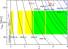
\includegraphics[width=0.8\columnwidth]{Figures/redshift_ladder.pdf}
	\caption[Spectral coverage of molecular emission lines]{The spectral coverage of CO, [CI] and H$_2$O emission lines as a function of redshift, showing the expected frequencies of certain lines in the region covered by ALMA's band-3 receiver. The green regions represent redshift windows where more than one line can be detected and yellow regions represent the redshifts where only one line can be detected. This figure was initially presented in \citealt{Weiss_2013}.}
	\label{fig:redshift_ladder}
\end{figure}

\section{Sample Creation}

\subsection{South Pole Telescope DSFGs}

A population of IR-bright SMGs selected at $1.4\,$mm were obtained from the South Pole Telescope - Sunyarv-Zel'dovich (SPT-SZ) survey (\citealt{Vieira_2010, Mocanu_2013, Everett_2020}) which covers approximately $2500\,$deg$^2$. The depth of this survey reaches $\sim 20\,$mJy at $1.4\,$mm. For a source to be included in our SPT sub-sample, we require that it has flux density above $25\,$mJy, corresponding to the sample of $81$ DSFGs presented in \citealt{Weiss_2013}, \citealt{Strandet_2016} and \citealt{Reuter_2020}.

The high flux density cuts imply that most IR-bright galaxies would not be intrinsically bright enough to be detected in this sub-sample without having been magnified from gravitational lensing. As shown by \citealt{Weiss_2013}, the average magnification of these sources are $\mu \sim 15$ (corresponding to intrinsic flux densities of $S_{1.4\,\textrm{mm}} = 1 - 3\,$mJy), which is similar to the flux densities of unlensed sources identified from blank field surveys at sub-mm/mm wavebands (e.g. \citealt{Coppin_2006, Pope_2006, Weiss_2009}), and are thus likely to be representative of this population albeit at higher observed redshifts.

During ALMA Cycle 0 \citealt{Weiss_2013} conducted a blind redshift survey for $26$ SPT sources with ALMA's band 3 receiver ($2.6 - 3.6\,$mm). In total $44$ line features were identified from $^{12}$CO, $^{13}$CO, [CI], H$_2$O and H$_2$O$^+$. $12$ sources had spectra with multiple clear line features, from which a unique redshift solution could be found from the ALMA scans alone; $11$ had a single line feature for which other spectroscopic or photometric measurements would be requied to constrain the redshift; and three sources for which no line features were observed. The same observing strategy was used during ALMA Cycle 1 by \citealt{Strandet_2016} to extend the redshift survey of \citealt{Weiss_2013} with an additional $15$ sources observed in ALMA band 3. For sources with a single CO line detection during Cycle 0, \citealt{Strandet_2016} present ALMA $1\,$mm (band 6) follow-up observations and, when still not satisfactory, follow-up observations were made with the First Light APEX Submillimetre Heterodyne receiver (FLASH; \citealt{Heyminck_2006}), the Swedish-ESO PI receiver (SEPIA; \citealt{Billade_2012}) and the Z-spec camera (\citealt{Naylor_2003}) onboard the Atacama Pathfinder Experiment (APEX) targeting CO and [CII] lines for those that remained unambiguous during Cycles 0 and 1. Lastly, \citealt{Reuter_2020} concluded the SPT redshift survey during ALMA Cycles 3, 4 and 7 by presenting spectra for the remaining $40$ of the total $81$ sources that had yet to be scanned. The culmination of these studies is a sample of $81$ SPT-selected DSFGs each with a spectroscopic redshift in the range $1.9 < z_{\textrm{spec}} < 6.9$ with a median redshift of $z_{\textrm{median}} = 3.9\pm0.2$ (\citealt{Reuter_2020}).

The SPT-DSFGs have photometric coverage that fully traces the SED peak and Rayleigh-Jeans (R-J) tail of the dust emission for all sources. Most of the SPT sample have coverage that spans at least observed wavelengths between $250\,\mu$m and $3\,$mm. This photometry includes flux densities measured at $250$, $350$ and $500\,\mu$m (\textit{Herschel}-SPIRE), $870\,\mu$m (APEX-LABOCA), $1.4$ and $2\,$mm (SPT) and $3\,$mm (ALMA). For a subset of $65$ sources, $100$ and $160\,\mu$m flux densities were measured with \textit{Herschel}-PACS. The photometric coverage of the sources covers a rest frame range of $86\,\mu$m $\lesssim \lambda_{\textrm{rest}} \lesssim 380\,\mu$m meaning that the peak of the dust emission at $\sim 100\,\mu$m is always constrained and the Rayleigh-Jeans tail is well sampled.

The complete set of photometric observations for the SPT DSFGs can be found in Appendix D of \citealt{Reuter_2020} including the estimated magnifications of each source due to gravitational lensing as measured from the lens modelling of \citealt{Spilker_2016}. In the 42 cases where a magnification could not be measured, the average value of $\mu = 5.5$ is assumed.

\subsection{The HerBS Sample}

A second sample used in this study comes from the \textit{Herschel} Bright Sources (HerBS; \citealt{Bakx_2018}) catalogue, a sample selected from the brightest high-redshift sources detected from the H-ATLAS project. Using the SED template derived by \citealt{Pearson_2013} to represent typical H-ATLAS sources, \citealt{Bakx_2018} estimated the redshift of each source and selected those that have a measured photometric redshift $> 2$ and are observed at a $500\,\mu$m flux density $> 80\,$mJy. Initially the sample consisted of $223$ sources, but having removed nearby galaxies and known blazars (\citealt{Negrello_2010, Lopez-Caniego_2013}), the HerBS sample is reduced to 209 sources. Presented with the catalogue are observations at $850\,\mu$m with the SCUBA-2 instrument for $203$ of these sources. Spectroscopic redshifts have been obtained for a selection of HerBS galaxies in the South Galactic Pole field, as part of the Bright Extragalactic ALMA Redshift Survey (BEARS: \citealt{Urquhart_2022, Bendo_2023, Hagimoto_2023}).

The BEARS spectral line survey started in ALMA Cycles 4 and 6 using the band 3 receiver of the Atacama Compact Array (ACA) and continued during Cycle 7 in bands 3 and 4 with the ALMA $12\,$m Array. \citealt{Urquhart_2022} targeted $85$ HerBS sources for CO line emission and presented spectroscopic measurements for $71$ sources associated with $62$ entries in the HerBS catalogue. The ALMA band 4 images with angular resolution of $\sim 2\,$arcsec revealed that only half of the fields contained just a single source, while several contained two or more objects with similar spectroscopic redshifts. This suggests either that the sources are formed from physically associated galaxies, or could be multiple images caused by gravitational lensing. For this study, we have retained the HerBS sources which are multiples in the ALMA images. In the cases where the HerBS source is deblended, we assume that the redshift of the group is the average spectroscopic redshift of all components, providing they are within $0.1$ of each other. If there is only a single redshift corresponding to one of the components (and the redshift corresponding to the integrated emission of all sources is not provided), we assumed the sources are physically connected and that the redshift of the one component is the redshift of the system. While \citealt{Bendo_2023} show that the brightest component (alphanumerically labelled A for each source) produces $< 80\%$ of the total emission at $2\,$mm, it is only in 4 fields (HerBS-56, -131, -138 and -146) that the spectroscopic redshift of a multiple system is assumed from a component that is not the brightest.

The photometry available for HerBS sources covers a similar range to the SPT sample: \textit{Herschel}-SPIRE ($250$, $350$, $500\,\mu$m), SCUBA-2 ($850\,\mu$m) and ALMA ($2$, $3\,$mm). The ALMA flux densities were serendipitously estimated from the continuum of the spectrosopic survey. We also include snapshot continuum observations in ALMA band 6 ($1.1 - 1.4\,$mm) for a selection of potentially "ultra-red" objects from the ALMARED survey (Jianhang Chen et al., in preparation) observed in the H-ATLAS (project 2018.1.00526.S). For sources where the reduced angular resolution of the ALMA beam resolves the HerBS source into multiple components, \citealt{Bendo_2023} report the integrated flux densities of all objects if they lie within twice the FWHM of the ALMA beam, or if they are connected by structures that are themselves detected at greater than 3$\sigma$ significance. We preferentially chose to use these integrated fluxes for each HerBS source if available, or failing this, combine the flux densities of individual components providing they are all detected.

The shorter selection wavelength compared to the SPT sample leads to a lower redshift distribution; the minimum and maximum redshifts are $z_{\textrm{min}} = 1.407$ and $z_{\textrm{max}} = 4.509$. The minimum photometric coverage for a HerBS galaxy is between rest frame wavelengths of $\sim 97\,\mu$m and $\sim 392\,\mu$m, which allows us to constrain the thermal peak and Rayleigh - Jeans tail of all galaxies in the sample, just as we can with the SPT DSFGs. The photometric coverage of the 30 HerBS galaxies used in the final sample (Section \ref{sec:restrictions_on_sample}) has been tabulated in Appendix \ref{app:HerBS_photometry}.

\subsection{Restrictions on Sub-samples}
\label{sec:restrictions_on_sample}

Across the two sub-samples there are $143$ galaxies with a spectroscopic redshift ($81$ SPT, $62$ HerBS/BEARS). However, as we are interested in measuring the galaxy-integrated dust emissivity spectral index of each source, which is characterized by the slope of the emission on the R-J side of the Planck function, we make it a requirement of the final samples that there are at least two observations at observed wavelengths greater than $1\,$mm for each galaxy. This has the effect of reducing the final sample of galaxies studied here to $109$ ($79$ SPT and $30$ HerBS/BEARS). While the fitting methods used in this study are the same for both sub-samples, we treat the two populations separately to highlight any potential differences that may result from the different selection wavelengths and flux limits. The redshift distributions of the two sub-samples is illustrated in Figure \ref{fig:spt_herbs_redshift}.

\begin{figure}
	\centering
	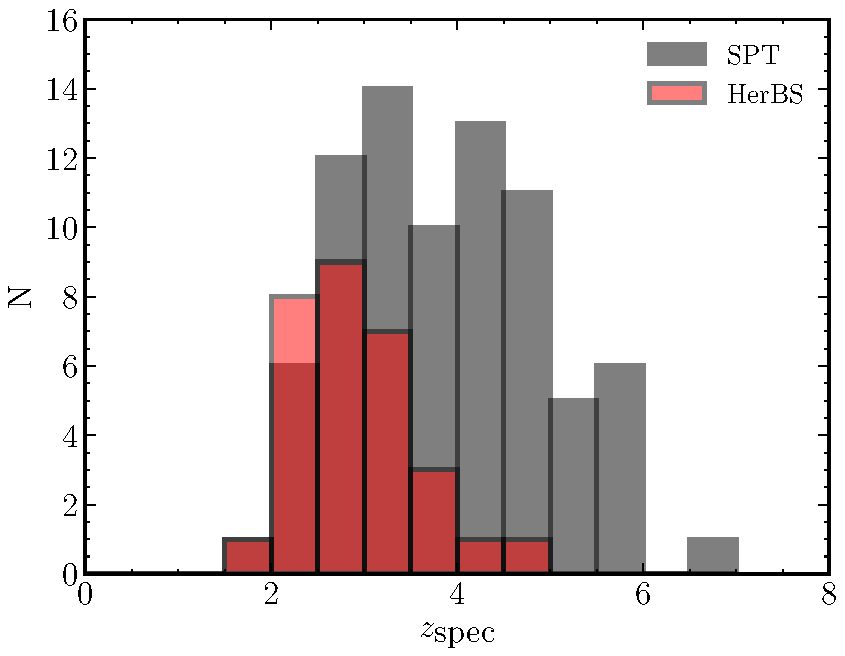
\includegraphics[width=0.8\columnwidth]{Figures/spt_herbs_redshift_distribution.pdf}
	\caption[Spectroscopic redshift distributions of HerBS and SPT-DSFG samples]{The spectroscopic redshift distributions for the SPT-DSFG (grey) and HerBS (red) samples.}
	\label{fig:spt_herbs_redshift}
\end{figure}

\section{Far-Infrared and Sub-mm Colours}
\label{sec:fir_submm_colours}

A first estimate on the average dust properties of the two samples can be made by comparing their far-IR/sub-mm colours (which we define as the ratio between two flux densities) with the predictions made using isothermal blackbody models. Previous studies have shown that far-IR colours can be useful proxies for dust properties (e.g. \citealt{Boselli_2010, Boselli_2012, Remy-Ruyer_2013, Smith_2019}) depending on the part of the far-IR spectrum that the colour samples. For example, smaller wavelengths involving the PACS and SPIRE flux densities are more sensitive to changes in the dust temperature, while longer wavelengths are more sensitive to variations in the dust emissivity spectral index. In Figure \ref{fig:spt_herbs_colour_redshift} we show a selection of colours using flux densities between $250\,\mu$m and $3\,$mm that progressively travel across the spectrum from sampling the peak of thermal dust emission to the R-J tail. Using an optically thin, isothermal modified blackbody model of the form $S_\nu \propto \frac{\nu^{\beta+3}}{e^{h \nu/kT} - 1}$, we predict the dependence of far-IR/sub-mm colour on redshift for three combinations of dust temperature, $T_{\textrm{dust}}$, and $\beta$ ([$T_{\textrm{dust}} = 30\,$K, $\beta = 2$], [$T_{\textrm{dust}} = 30\,$K, $\beta = 1.8$] and [$T_{\textrm{dust}} = 40\,$K, $\beta = 2$]). It can be seen that the assumed dust temperature has a significant effect on the location of the SED evolution for all colours, while it is noticable that a change in $\beta$ has a substantially larger effect on the observed colours at the longest wavelengths. 

\begin{figure}
    \centering
    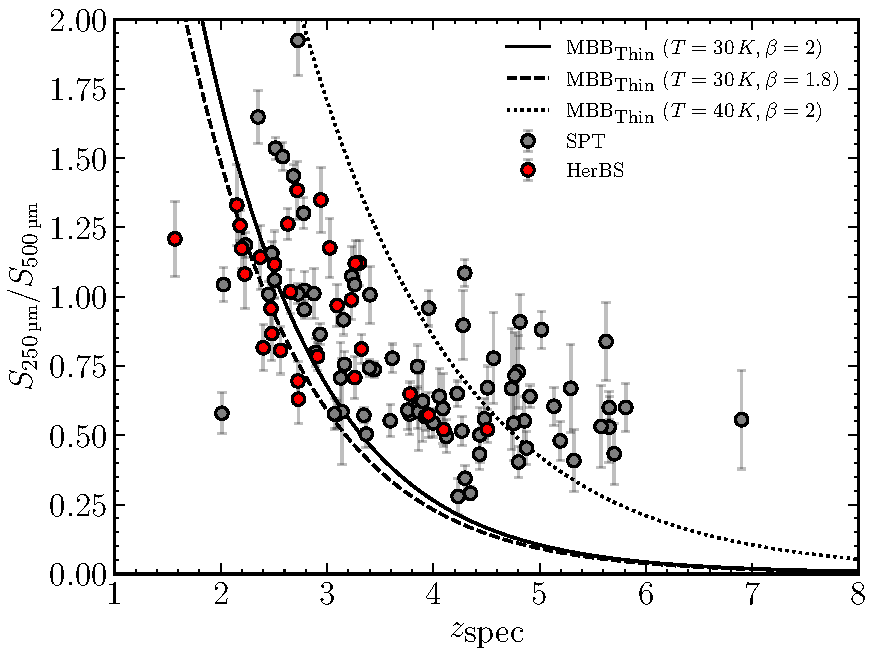
\includegraphics[width=0.55\columnwidth,height=0.29\textheight]{Figures/spt_herbs_colour_250_500.pdf}
    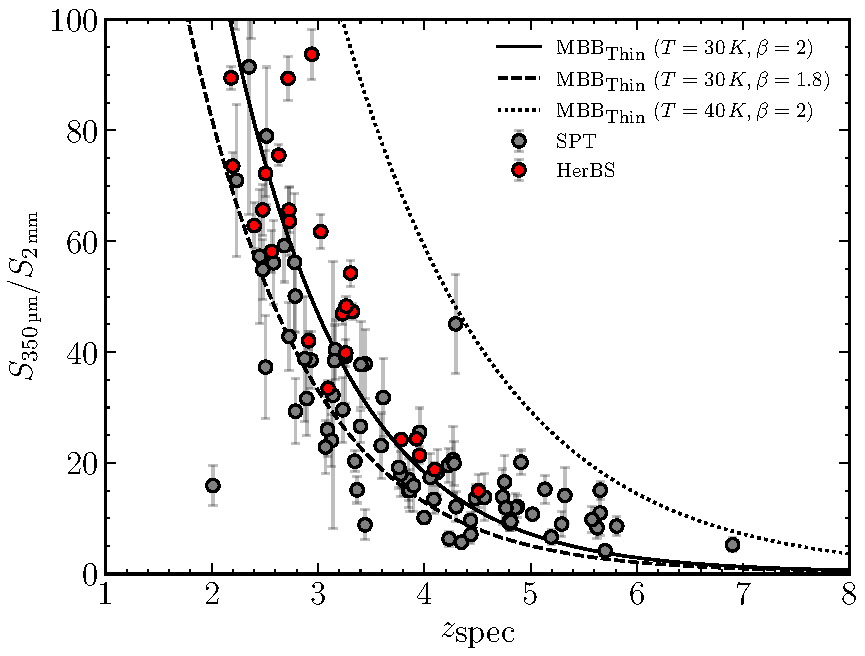
\includegraphics[width=0.55\columnwidth,height=0.29\textheight]{Figures/spt_herbs_colour_350_2000.pdf}
    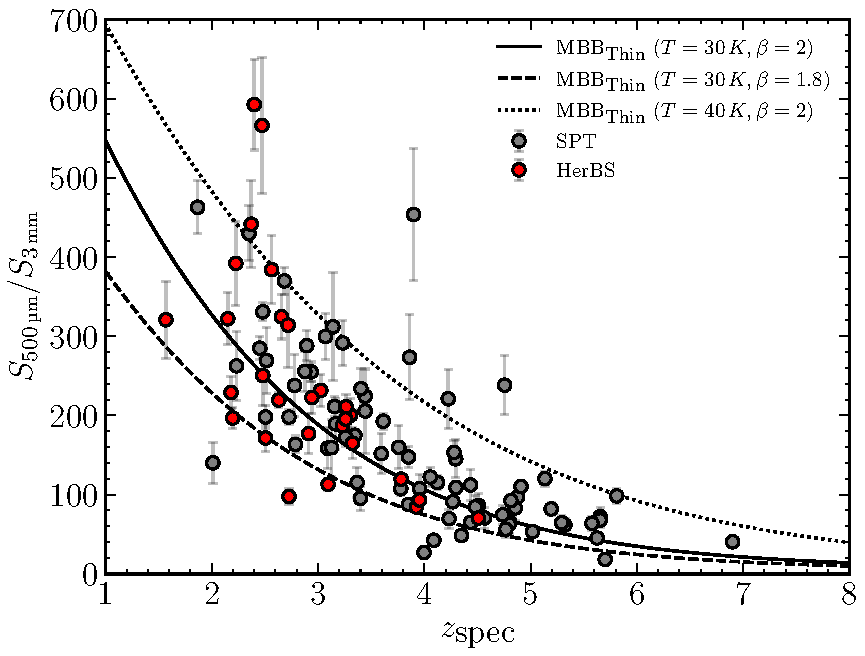
\includegraphics[width=0.55\columnwidth,height=0.29\textheight]{Figures/spt_herbs_colour_500_3000.pdf}
    \caption[Colours of HerBS and SPT sources as a function of redshift]{Colour-redshift plots of $S_{250}/S_{500}$, $S_{350}/S_{2\,\textrm{mm}}$ and $S_{500}/S_{3\,\textrm{mm}}$ against spectroscopic redshift. The SPT sources are illustrated with grey circles and the HerBS sample as red circles. The predictions from three modified blackbody models assuming optically thin dust ([$T_{\textrm{dust}} = 30\,$K, $\beta = 2$], [$T_{\textrm{dust}} = 30\,$K, $\beta = 1.8$] and [$T_{\textrm{dust}} = 40\,$K, $\beta = 2$]) are plotted as solid, dashed and dotted black lines, respectively.}
    \label{fig:spt_herbs_colour_redshift}
\end{figure}

Assuming for now that the dust emissivity index is well represented by $\beta \sim 2$ for all galaxies, then the far-IR/sub-mm colours of most sources can be explained by a range of dust temperatures between $T_{\textrm{dust}} = 30 - 40\,$K assuming optically thin dust emission. There are notable exceptions, including a selection of SPT sources with high $S_{250}/S_{500}$ and sources from both samples with high $S_{500}/S_{3\,\textrm{mm}}$. At first this might suggest sources with large dust temperatures and/or high values of $\beta$, but other common culprits could be leading to these deviations from the bulk population. The most likely are the uncertainties on the flux density measurements or biases due to combining photometry from different facilities. We note that our galaxies contain a combination of photometry obtained from single-dish observations (e.g. \textit{Herschel}, JCMT and SPT) and from the interferometer, ALMA. With their varying angular resolutions, emission observed with one instrument may be missed by another. In particular, we might expect that when ALMA resolves the single sources observed in the \textit{Herschel} wavebands into multiple components, some emission is lost giving the impression of higher far-IR/sub-mm colours and thus higher dust temperatures and/or higher $\beta$. In general, however, the SPT and HerBS galaxies occupy similar regions of the colour-redshift space, suggesting that the intrinsic dust properties of the two samples are likely to be similar. Given the scatter observed around the MBB models, it appears unlikely that a single value of dust temperature and $\beta$ represents the observed SED of each galaxy equally well. This would suggest that a single dust model assuming a constant $\beta$ is unlikely to explain the variety of SEDs observed among the two sub-samples. We are, however, interested in ascertaining a single galaxy-integrated $\beta$, thus we must turn to fitting the observed SEDs individually to measure their dust properties.

\section{SED Fitting of DSFGs}
\label{sec:sed_fitting}

We model the far-IR to millimeter spectra of our galaxies by fitting a single modified blackbody model, combined with a mid-IR power law to all sources. In the far-IR to mm regime the SED is dominated by a modified Planck function that represents the cold dust reservoir from which most of the mass of interstellar dust in the ISM is contained. This "cold" dust resides in the diffuse ISM and is heated by the ambient interstellar radiation field. A lower fraction of dust by mass radiates at hotter temperatures, heated by nearby star-forming regions, young OB-like stars or AGNs which contribute substantially to a galaxy's IR luminosity and dominates the emission at rest frame wavelengths $\lesssim 70\,\mu$m. This mid-IR component can be approximated using a power law of dust temperatures of the form $S_\nu \propto \nu^{-\alpha}$, where a lower value of $\alpha$ represents a higher fraction of emission emananting from sources other than the cold reservoir of dust, and higher values asymptotically tending towards a modified blackbody, representing a single temperature of dust.

The modified blackbody form is a direct result of the radiative transfer equation, $\frac{dI_\nu}{ds} = -\kappa_\nu \rho I_\nu + j_\nu \rho$, where $\kappa_\nu$ represents the opacity of the dust, $\rho$ is the density, $j_\nu$ represents the emissivity of the dust and $I_\nu$ is the spectral radiance (per unit area). If we define the source function, $S_\nu$ as $j_\nu/\kappa_\nu$ and the frequency dependent optical depth as $d\tau_\nu = -\kappa_\nu \rho ds$, then the radiative transfer equation becomes $\frac{dI_\nu}{d\tau_\nu} = I_\nu - S_\nu = I_\nu - B_\nu$, where we have used the fact that at local thermal equilibrium (LTE) the source function is equal to the Planck function, $B_\nu(T)$. The solution to the radiative transfer equation takes the form $I_\nu = (1 - e^{-\tau_\nu}) B_\nu(T)$. Given that the spectral radiance is proportional to the flux density at a given frequency, we can rewrite this as the modified blackbody model

\begin{equation}
	S_{\nu, \textrm{obs}} =  
	\begin{cases}
	 	\frac{\Omega}{(1+z)^3} (1- e^{-\tau_\nu}) B_\nu(T_{\textrm{dust}}), & \nu \le \nu_{\rm c} \\
	 	 N \nu^{-\alpha}, & \nu > \nu_{\rm c} \\
	\end{cases}
	\label{eq:modified_blackbody_omega}
\end{equation}

\noindent where $\Omega$ represents the solid angle subtended by the galaxy and we have included the power law form at mid-IR wavelengths. $N$ represents a normalization for the power law which is tied to the normalization of the blackbody. The value of $\nu_{\rm c}$ is the frequency at which the gradient of the MBB is equal to the value of $\alpha$. The solid angle, $\Omega$, is defined as $\frac{A(1+z)^4}{D_{\rm L}^2}$, where $A$ is the area of the source and $D_{\rm L}$ represents the luminosity distance at the redshift of the galaxy. 

The optical depth, $\tau$, is defined as the product of dust surface mass density, $\Sigma_{\textrm{dust}} = M_{\textrm{dust}}/A$ and the dust opacity, $\kappa_\nu$, but is often assumed to take the form of a power law, $(\nu/\nu_1)^\beta$, where $\nu_1$ represents the frequency at which the optical depth equals unity, and thus marks the transition between optically thick and optically thin dust. We can also describe the emissivity of the dust grains per unit mass, $\kappa_\nu$, in a similar way, using a power law of the form $\kappa_\nu = \kappa_0(\nu/\nu_0)^\beta$, where $\kappa_0$ is the emissivity of the grains per unit mass at some reference frequency $\nu_0$. Hereafter, we shall adopt $\kappa_0 = 0.077\,$m$^2$kg$^{-1}$ at $\nu_0 = 353\,$GHz ($\lambda_0 = 850\,\mu$m, \citealt{Dunne_2000, James_2002}), like we did in the previous Chapter.

Upon substituting for optical depth, we find 

\begin{equation}
	S_{\nu, \textrm{obs}} =  
	\begin{cases}
		\frac{\mu A (1+z)}{D_{\rm L}^2} \Big(1- e^{-\frac{M_{\textrm{dust}}\kappa_\nu}{A}}\Big) B_\nu(T_{\textrm{dust}}), & \nu \le \nu_{\rm c} \\
		\mu N \nu^{-\alpha}, & \nu > \nu_{\rm c} \\
	\end{cases}
\end{equation}

\noindent where we have included a term, $\mu$, accounting for the possibility of gravitational lensing. This allows us to determine intrinsic masses and luminosities. For galaxies where there is no evidence of gravitational lensing, this value defaults to $\mu = 1$.

The final amendment to the MBB models is to account for the heating of the dust due to the ambient temperature of the Cosmic Microwave Background (CMB). At high redshifts the CMB becomes a non-negligible source of heating, which unaccounted for in the model, could bias estimates of the dust temperature and dust emissivity index. When the CMB temperature at the redshift of the galaxy is a significant fraction of the cold dust temperature of the ISM within the galaxy, then we observe a change in the shape of the far-IR/sub-mm SED (\citealt{daCunha_2013}, see also \citealt{Zhang_2016} for the influence of the CMB on the measurement of structural and dynamical properties). At local thermal equilibrium, the increase in the ISM temperature due to CMB heating at higher redshifts ($T_{\textrm{CMB}} = T_{\textrm{CMB}, 0}(1+z)$, where $T_{\textrm{CMB}, 0}$ is the temperature of the CMB today, $2.72\,$K) has two competing effects on the observed dust SED. First, the dust continuum emission is boosted by the increased temperature of the CMB; and second, the increased temperature creates a stronger background from which we observe the dust continuum. The CMB-adjusted blackbody model is now given by 

\begin{equation}
	S_{\nu, \textrm{obs}} =  
	\begin{cases}
		f_{\textrm{CMB}}\frac{\mu A (1+z)}{D_{\rm L}^2} \Big(1- e^{-\frac{M_{\textrm{dust}}\kappa_\nu}{A}}\Big) B_\nu(T_{\textrm{dust}}(z)), & \nu \le \nu_{\rm c} \\
		f_{\textrm{CMB}} \mu N \nu^{-\alpha}, & \nu > \nu_{\rm c} \\
	\end{cases}
	\label{eq:modified_blackbody_general_opacity_a_cmb}
\end{equation}

\noindent where we have made two changes. First, the prefactor $f_{\textrm{CMB}}$ denotes the fraction of the total dust emission that is observed against the background of the CMB and is given by Equation 18 of \citealt{daCunha_2013}; $f_{\textrm{CMB}} = \frac{S_\nu^{\textrm{observed}}}{S_\nu^{\textrm{intrinsic}}} = 1 - \frac{B_\nu[T_{\textrm{CMB}}(z)]}{B_\nu[T_{\textrm{dust}}(z)]}$. Second, we have redefined the dust temperature to be a function of redshift, $T_{\textrm{dust}}(z)$, and is given by Equation 12 of \citealt{daCunha_2013}; $T_{\textrm{dust}}(z) = [T_{\textrm{dust}, 0}^{4+\beta} + T_{\textrm{CMB}, 0}^{4+\beta} ((1+z)^{4+\beta} - 1)]^{\frac{1}{4+\beta}}$, where $T_{\textrm{dust}, 0}$ is the dust temperature at a redshift of zero. Note that in all future references of the dust temperature of a galaxy, we refer to the luminosity-weighted, CMB-corrected temperature as defined above, unless otherwise stated.

In this general opacity form of the modified blackbody there are up to four free parameters describing the dust properties of the galaxy: the dust mass, $M_{\textrm{dust}}$, the characteristic dust temperature, $T_{\textrm{dust}}$, the radial size of the source, $r$ (which we use to define the source area, $A$), and the dust spectral index, $\beta$. As mentioned previously, some of the SPT sources have intrinsic size measurements from lens modelling in \citealt{Spilker_2016} - although caution should be exercised when using these estimates as the size is measured at a particular wavelength (in this case at $870\,\mu$m with ALMA imaging), and it is unlikely to be the same at all wavelengths due to differential lensing. We assume no differential lensing and take the effective radii as the size of the dust continuum region for the fraction of SPT galaxies modelled in \citealt{Spilker_2016}. These measurements suggest that the sizes of the sub-mm emitting region is typically $\sim 1\,$kpc. All the remaining SPT and HerBS sources without known sizes require an alternative way of constraining the dust opacity. We recall the two definitions of the optical depth given above. By equating the two forms of $\tau$, $\Sigma_{\textrm{dust}}\kappa_\nu$  and $(\nu/\nu_1)^\beta$, we can find an alternative definition that reformulates the intrinsic size into an observed parameter. This is given by the transitional frequency, $\nu_1 = \nu_0 (\kappa_0\Sigma_{\textrm{dust}})^\beta = \nu_0 (\kappa_0M_{\textrm{dust}}/A)^\beta$.

We estimated the properties of the dust using three separate models. In the first, we make the simple approximation that the dust is optically thin at all wavelengths, $\tau_\nu \ll 1$, which simplifies the self opacity term from $(1 - e^{-\tau_\nu})$ to $\tau_\nu$, and removes the necessity for defining the size of the continuum emission

\begin{equation}
	S_{\nu, \textrm{obs}} =  
	\begin{cases}
		f_{\textrm{CMB}}\frac{\mu (1+z)}{D_{\rm L}^2} M_{\textrm{dust}} \kappa_\nu B_\nu(T_{\textrm{dust}}(z)), & \nu \le \nu_{\rm c} \\
		f_{\textrm{CMB}}\mu N \nu^{-\alpha}, & \nu > \nu_{\rm c} \\
	\end{cases}
    \label{eq:modified_blackbody_optically_thin}
\end{equation}

Given how high the dust masses are expected to be for the \textit{Herschel} and SPT DSFGs (and the dust is packed into a small region, e.g. \citealt{Ikarashi_2017}), it is not unreasonable to expect that the dust might be optically thick at wavelengths probed by our photometry (e.g. \citealt{Conley_2011, Casey_2019, Cortzen_2020}). For this reason, the other two models assume that dust becomes optically thick at wavelengths below $\lambda_1 = 100\,\mu$m or $200\,\mu$m (e.g. \citealt{Blain_2003, Draine_2006, Conley_2011, Rangwala_2011, Greve_2012, Casey_2014a, Spilker_2016, Casey_2019, Cooper_2022, Drew_2022}). The SPT sources that have size measurements have an additional model using the derived value of $A$, which is used as a means of comparison.

The lensing magnifications, $\mu$, are required to calculate the intrinsic mass and luminosity of the dust. We take the the lensing magnifications to be those quoted in the lens modelling of \citealt{Spilker_2016} for the SPT-DSFGs and from the well-studied correlation between CO luminosity and line width (e.g. \citealt{Bothwell_2013, Dannerbauer_2017, Neri_2020}) as determined by \citealt{Urquhart_2022}, building on the work of \citealt{Harris_2012}, for the HerBS galaxies. The effect of gravitational lensing is to amplify the apparent CO luminosity, while the line width is unaffected. Thus, the offset from the relationship defined by a population of known unlensed sources can then be used to estimate the value $\mu$. In the case of the HerBS sources in this study, the magnification factors are in the range $1 - 50$ and the median is $\mu_{\textrm{median}} = 5.3$. The SPT-DSFGs range in magnification factors from $1$ to $33$, with a median value $\mu_{\textrm{median}} = 5.5$, which is assumed for all SPT sources not included in the study of \citealt{Spilker_2016}. 

Finally, during the SED fitting we assumed flat priors on all the free parameters and added calibration errors in quadrature with the flux density uncertainties at each wavelength, in the same manner as we described in Section \ref{sec:phot_z_Herschel}. We assumed absolute calibrations of $7\%$ (\textit{Herschel}-PACS), $5.5\%$ (\textit{Herschel}-SPIRE), $5\%$ (SCUBA-2), $12\%$ (APEX-LABOCA), $7\%$ (SPT) and $10\%$ (ALMA). The best fitting SED was determined from a Markov Chain Monte Carlo (MCMC) algorithm using the \texttt{emcee} package (\citealt{Foreman-Mackey_2013}), and the $1\sigma$ uncertainties quoted from the $16$th and $84$th percentiles of the posterior distribution for each dust parameter.

For consistency across the literature, we have conformed to the "best practices" outlined in \citealt{Drew_2022}. These recommendations aim to make cross-referencing comparisons between studies easier and provide a set of guidelines that allows future studies to compare the dust properties of different galaxy populations coherently. In brief, these guidelines are: 

\begin{itemize}
	\item Galaxies that lack photometric coverage should not be fit with models containing more free parameters than data. In the case of the MBB models used here, the maximum number of free parameters are five for the general opacity model ($M_{\textrm{dust}}$, $T_{\textrm{dust}}$, $\beta$, $\alpha$ and $r$/$\lambda_1$) and four when using the optically thin approximation ($M_{\textrm{dust}}$, $T_{\textrm{dust}}$, $\beta$ and $\alpha$), whereas there are no sources with fewer than six photometric constraints in the SPT-DSFG sample, and no sources with fewer than five in the HerBS sample.
	\item The number of free parameters should vary depending on the available photometric constraints. For parameters that are not well constrained by photometric data, these values should be fixed. In this study, we assume flat priors given that we do not know suitable prior distributions to explain our sub-samples and this will not be inferred through Hierarchical Bayesian fitting (see \citealt{Lamperti_2019} for an example of this method). However, in accordance with the best practices, we fix the wavelength below which the dust is optically thick, if the dust continuum sizes are unknown, in order to constrain the dust opacity. This is important in this study where the photometry alone does not constrain $\tau$ well, and we do not have independent measurements for the dust column density of these sources. 
	\item Poorly sampled SEDs that have no spatially-resolved dust continuum observations should focus on constraining the rest-frame peak wavelength $\lambda_{\textrm{peak}}$ rather than the dust temperature. As will be mentioned later, we do not consider the dust temperature obtained from our fits to be the true temperature of the dust, but rather a single, luminosity-weighted value that describes the bulk of the dust by mass in the ISM. In Section \ref{sec:dust_temperature_evolution} we shall define an alternative dust temperature for the \textit{Herschel} and SPT galaxies as defined by their peak wavelength, which is less biased by the choice of SED model.
\end{itemize}

\section{Results of SED Fitting}

\subsection{Example SEDs - SPT0002-52 and HerBS-11}

In Figure \ref{fig:example_SEDs} we show the joint posterior distributions from the fitting of the first source alphanumerically in the two sub-samples, SPT0002-52 and HerBS-11. We include the fitting parameters $M_{\textrm{dust}}$, $T_{\textrm{dust}}$ and $\beta$, as well as derived quantities, the IR luminosity ($8 - 1,000\,\mu$m), $L_\textrm{IR}$, and the wavelength where the dust emission peaks, $\lambda_\textrm{peak}$. Neither galaxy has an independent measurement for its continuum emission size, so we have illustrated the optically thin, $\lambda_1 = 100\,\mu$m and $\lambda_1 = 200\,\mu$m models (filled contours, solid contours and dashed contours, respectively). The best fitting SEDs for all sources, including SPT0002-52 and HerBS-11, can be found in Appendices \ref{app:HerBS_SEDs} and \ref{app:SPT_DSFG_SEDs}. As we predicted from the general population of far-IR/sub-mm colours in Section \ref{sec:fir_submm_colours}, the two sources have similar posterior distributions that sample similar ranges in the parameter space. The only significant difference between the two figures is the extended tail to the IR luminosity for HerBS-11. This is a direct result of not having PACS observations that help to constrain the mid-IR power law, whereas there are observations at these wavelengths for SPT0002-52. We can see that the measurement of the dust mass and dust temperature are unaffected by the lack of PACS detections, which are useful in constraining the contribution from hotter dust at such high redshifts, suggesting that we still constrain the cold dust component of these galaxies well. 

\begin{figure}
	\centering
	\includegraphics[width=0.7\columnwidth]{Figures/spt_example_contours.pdf}
	\includegraphics[width=0.7\columnwidth]{Figures/herbs_example_contours.pdf}
	\caption[Posterior distributions for SPT0002-52 and HerBS-11]{The joint posterior distributions of SPT0002-52 (top) and HerBS-11 (bottom). The fitting parameters illustrated are the dust mass, the dust temperature and $\beta$. The derived parameters, IR luminosity ($8 - 1000\,\mu$m) and the peak wavelength, $\lambda_\textrm{peak}$ are also included. The optically thin, $\lambda_1 = 100\,\mu$m and $\lambda_1 = 200\,\mu$m models are shown as filled contours, solid contours and dashed contours, respectively.}
	\label{fig:example_SEDs}
\end{figure}

Both galaxies show offsets in the dust mass and dust temperature posterior distributions, depending on the choice of model. This is not observed for $\beta$ or the derived quantities. We discuss these differences in more detail in the next section.

\subsection{Comparison between Optically Thin and General Opacity Models}
\label{sec:comparison_optically_thin_and_general_opacity}

A singular galaxy's posterior distributions may not be particularly informative if the photometric constraints allow for a wide variety of SED shapes, however, by stacking the posterior distributions for all sources in a sub-sample, we can determine preferred regions of parameter space, estimate the average dust properties for a population of galaxies, and observe how diverse the population is. 

Figure \ref{fig:stacked_posteriors} shows the stacked posterior distributions for SPT galaxies (top, black histograms) and HerBS galaxies (bottom, red histograms). The parameters are the same as those plotted in Figure \ref{fig:example_SEDs}, but with the magnification factors included in the dust mass and luminosity estimates. We make this choice as it more closely resembles the set of observable properties; without the lensing magnifications, the posterior distributions are not as smooth and do not tell us about the parameter space that is explored by samples selected in \textit{Herschel} and SPT surveys.

\begin{figure}
	\centering
	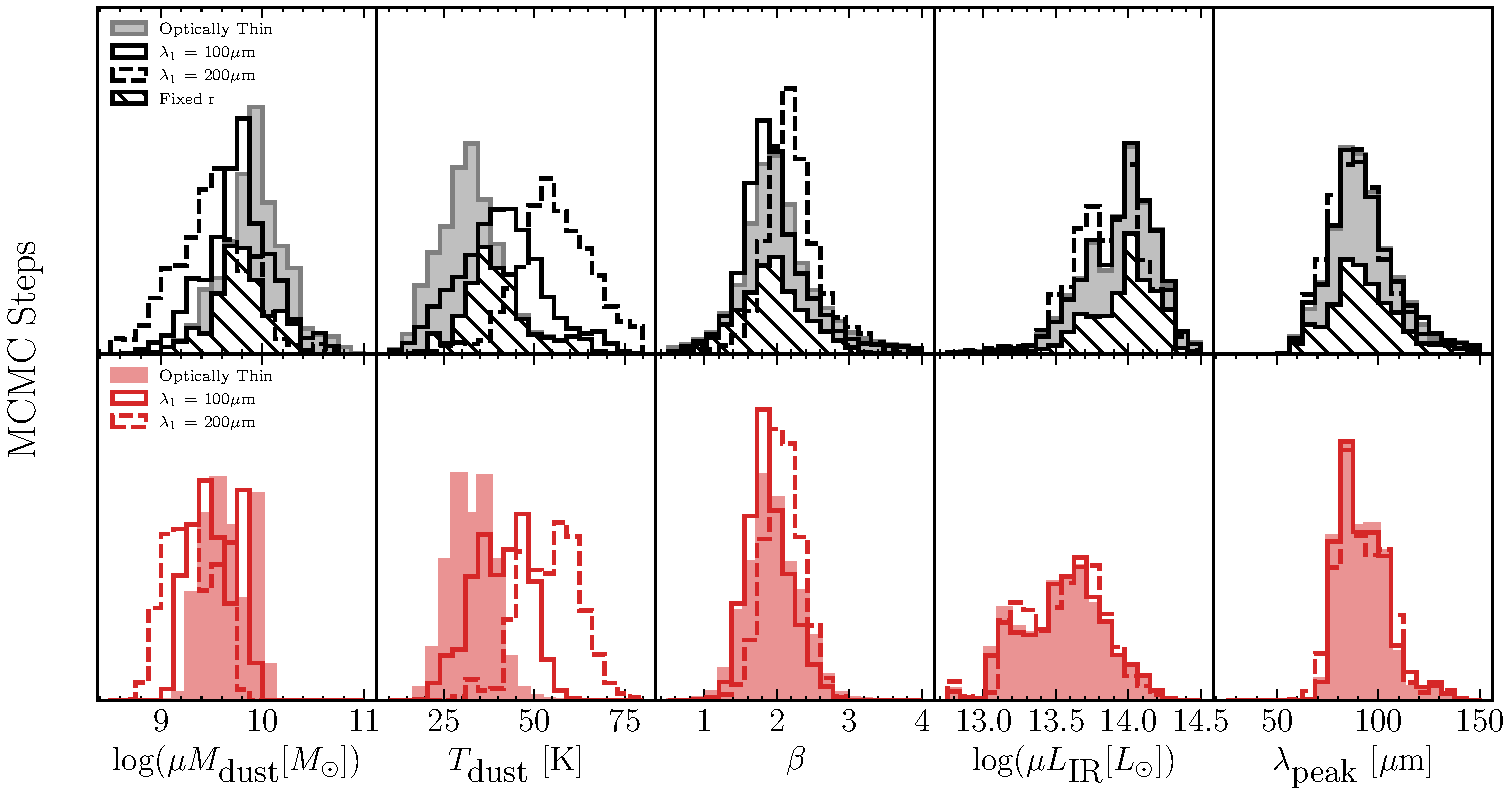
\includegraphics[width=\columnwidth]{Figures/stacked_posterior.pdf}
	\caption[Stacked posterior distributions for each MBB model]{The stacked posterior distributions of log($\mu M_{\textrm{dust}}$), $T_{\textrm{dust}}$, $\beta$, log($\mu L_{\textrm{IR}}$) and $\lambda_{\textrm{peak}}$ for SPT (top panels) and HerBS galaxies (bottom panels). The posterior distribution for each MBB model is illustrated as follows: optically thin (shaded), $\lambda_1 = 100\,\mu$m (solid line), $\lambda_1 = 200\,\mu$m (dashed line) and fixed continuum size (hatched).}
	\label{fig:stacked_posteriors}
\end{figure}

The median values and the $16$th and $84$th percentiles of the probability distributions are listed in Table \ref{tab:parameter_results}. The main parameter of interest, $\beta$, covers only a range of $0.2$ for the three models, showing that it is relatively insensitive to our assumptions about the dust opacity. This conclusion was also found in a recent study of DSFGs selected from the z-GAL NOEMA spectroscopic redshift survey by \citealt{Ismail_2023}. Despite the small range, the model with the highest value of $\lambda_1$, also gives the highest value of $\beta$, a trend that has been observed previously (e.g. \citealt{McKay_2023}). In this study of $870\,\mu$m selected galaxies in GOODS-S, the median $\beta$ systematically increased from $1.78$ and $1.80$ for their optically thin and $\lambda_1 = 100\,\mu$m MBB models, to $2.02$ for $\lambda_1 = 200\,\mu$m. It has recently been suggested that at high redshift a value of $\beta > 2$ might be appropriate for most galaxies (e.g. \citealt{Casey_2019, Casey_2021, Cooper_2022}), but this might suggest that the reason for their anomalous $\beta$ values are their common use of high $\lambda_1$ values. Considering this, future studies concerning the evolution of the dust SED with redshift or comparing DSFGs in the literature, should consider whether $\lambda_1$ is consistent for all sources, and/or should have its own freedom to evolve.

\begin{table}
    \centering
    \begin{tabular}{p{3.5cm}p{2.5cm}p{2.5cm}p{2.5cm}}
	\hline
	\hline
	Parameter & Optically Thin & $\lambda_1 = 100\,\mu$m & $\lambda_1 = 200\,\mu$m \\
	\hline
	\hline
	& \multicolumn{3}{c}{SPT} \\
	\hline
	log($\mu M_{\textrm{dust}} [$M$_\odot]$) & $9.92_{-0.31}^{+0.30}$ & $9.77_{-0.34}^{+0.31}$ & $9.49_{-0.41}^{+0.37}$ \\
	$T_{\textrm{dust}}$ [K] & $32.07_{-8.44}^{+8.43}$ & $40.77_{-11.77}^{+10.90}$ & $55.63_{-9.28}^{+11.20}$ \\
	$\beta$ & $1.98_{-0.39}^{+0.54}$ & $1.91_{-0.32}^{+0.50}$ & $2.18_{-0.30}^{+0.38}$ \\
	log($\mu L_{\textrm{IR}} [$L$_\odot]$) & $13.98_{-0.31}^{+0.19}$ & $13.99_{-0.30}^{+0.19}$ & $13.89_{-0.27}^{+0.23}$ \\
	$\lambda_{\textrm{peak}}$ [$\mu$m] & $90.70_{-12.72}^{+17.33}$ & $90.70_{-13.02}^{+18.36}$ & $89.28_{-13.39}^{+15.21}$ \\
	
	\hline
	& \multicolumn{3}{c}{HerBS} \\
	\hline
	
	log($\mu M_{\textrm{dust}} [$M$_\odot]$) & $9.62_{-0.22}^{+0.30}$ & $9.49_{-0.22}^{+0.31}$ & $9.30_{-0.26}^{+0.33}$ \\
	$T_{\textrm{dust}}$ [K] & $32.73_{-5.92}^{+5.85}$ & $41.16_{-8.20}^{+7.48}$ & $55.18_{-9.23}^{+7.25}$ \\
	$\beta$ & $1.92_{-0.32}^{+0.39}$ & $1.85_{-0.25}^{+0.34}$ & $2.08_{-0.25}^{+0.26}$ \\
	log($\mu L_{\textrm{IR}} [$L$_\odot]$) & $13.55_{-0.37}^{+0.27}$ & $13.57_{-0.37}^{+0.26}$ & $13.57_{-0.34}^{+0.25}$ \\
	$\lambda_{\textrm{peak}}$ [$\mu$m] & $90.03_{-9.28}^{+12.70}$ & $90.36_{-9.46}^{+13.42}$ & $89.96_{-9.46}^{+14.92}$ \\
	\hline
    \end{tabular}
	\caption[Median values of far-IR to mm SED parameters]{The median and 1$\sigma$ errors (estimated from the 16th, 50th and 84th percentiles of the stacked posterior distribution) for the parameters presented in Figure \ref{fig:stacked_posteriors}.}
    \label{tab:parameter_results}
\end{table}

As we observed with SPT0002-52 and HerBS-11, the assumption that the dust is optically thin or thick does have a large effect for dust masses and dust temperatures. There is a clear trend to higher dust temperatures with increasing $\lambda_1$, with differences of approximately $10\,$K and $20\,$K on average between the optically thin and $\lambda_1 = 100\,\mu$m and $\lambda_1 = 200\,\mu$m general opacity models, respectively. Given the inverse correlation between dust mass and dust temperature ($M_\textrm{dust} \propto S_\nu T_\textrm{dust}^{-1}$ for dust masses measured from the Rayleigh-Jeans regime, \citealt{Casey_2014b}), dust masses decrease by approximately $0.1\,$log($\mu M_\odot$) and $0.4\,$log($\mu M_\odot$) from the optically thin model to the $\lambda_1 = 100\,\mu$m and $\lambda_1 = 200\,\mu$m models, respectively. There is no significant difference in the IR luminosities or peak wavelengths between models.

Included in Figure \ref{fig:stacked_posteriors} are the posterior probability distributions for the subset of SPT galaxies where we had estimates of the area of the dust region (hatched histograms). Providing that these galaxies do not represent a biased selection of the total sample, their dust properties are based on a self-consistent dust model that is useful for comparing with the remaining sources. Generally, we find that the distributions for each dust parameter agree best with the optically thin and $\lambda_1 = 100\,\mu$m model, but not always with $\lambda_1 = 200\,\mu$m, suggesting that such a high value may not be appropriate for all SPT detected galaxies. Using the equation relating $\lambda_1$ with the dust surface mass density, $\Sigma_\textrm{dust}$, provided earlier, we find a median value of $\lambda_1 = 88\,\mu$m for these sources, with a $16$th to $84$th percentile range of $44 - 224\,\mu$m. However, this calculation depends heavily on the value assumed for $\kappa_\nu$, whch is notoriously uncertain (\citealt{Clark_2016}). The probability distributions for the optically thin model are a good match to those estimated from the subset of galaxies with measured values of $A$, and therefore the parameter estimates quoted herein have been derived using the optically thin model. An added benefit is that the optically thin, isothermal model is widely used in the literature and makes comparisons across studies easier (e.g. \citealt{Magdis_2012, Simpson_2017, Lamperti_2019, Dudzeviciute_2020, Valentino_2020a, daCunha_2021}).

To determine whether the offsets in the assumed model are the same for all galaxies, we show the median values of the parameters estimated from the optically thin model against those estimated from the general opacity models in Figure \ref{fig:comparison_optically_thin_general_opacity}. These panels show the size of the systematic error we might expect if, contrary to our first choice model, the dust is actually optically thick. Here we observe a clear trend in the dust masses and dust temperatures, such that the difference between assuming optically thin and optically thick dust is most extreme for low masses and high temperatures.

\begin{figure}
	\centering
	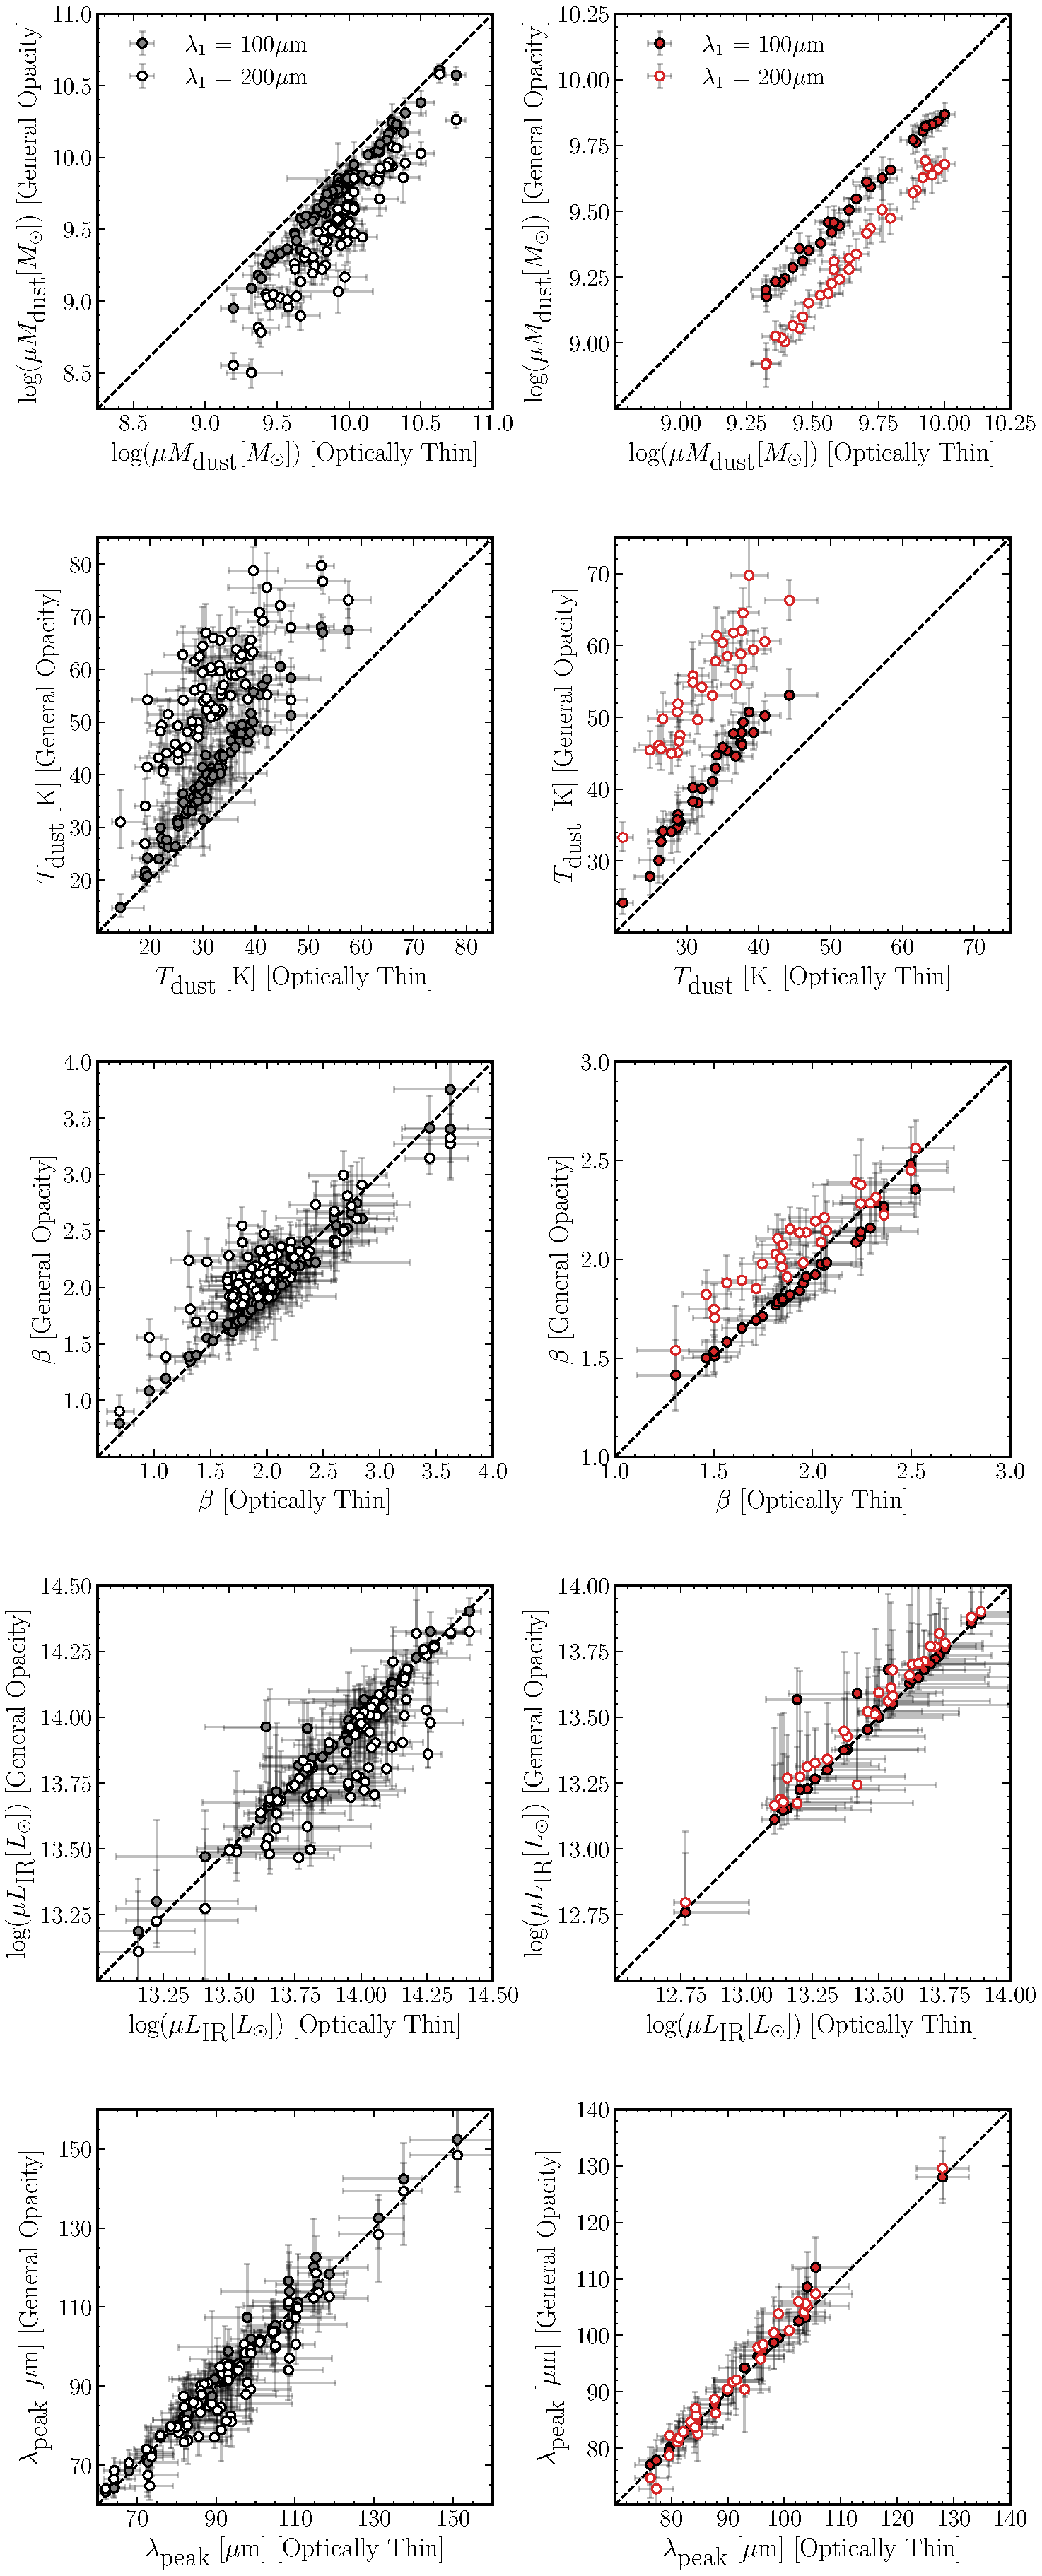
\includegraphics[height=0.9\textheight]{Figures/Figure_4_6.pdf}
	\caption[Comparison of best fitting optically thin and general opacity parameters]{Comparison between the optically thin model and the general opacity models in predicting the dust properties of SPT (left column) and HerBS (right column) galaxies. The general opacity models are shown as filled and open circles for $\lambda_1 = 100\,\mu$m and $200\,\mu$m, respectively.}
	\label{fig:comparison_optically_thin_general_opacity}
\end{figure}

\subsection{The $\beta$-Dust Temperature Degeneracy}

Due to correlated errors between the dust temperature and $\beta$, a well established artificial anti-correlation is observed when fitting. Such a degeneracy between the two parameters has been observed for a wide variety of sources in which an isothermal MBB might be used, including dust clouds in the Galaxy to integrated values over whole extragalactic sources, as we apply the model here (e.g. \citealt{Dupac_2003, Desert_2008, Paradis_2010, Schnee_2010, Veneziani_2010, Bracco_2011, Galametz_2012, Paladini_2012, Smith_2012, Lamperti_2019, daCunha_2021}). While many studies report the presence of a correlation between $T_\textrm{dust}$ and $\beta$, it has also been shown that an artificial correlation can be produced from fitting SEDs with large measurement uncertainties (\citealt{Shetty_2009a, Kelly_2012, Juvela_2012a}), and from assuming a constant temperature in scenarios where the reality is that there are multiple dust temperatures along the line of sight to the observer (\citealt{Shetty_2009b, Juvela_2012b}). As a result, it is still debated whether this common correlation represents a true relationship between these properties of the dust, or whether it is artificially produced.

Figure \ref{fig:beta_t_correlation} shows that there is a negative correlation between the measured values of $\beta$ and dust temperature for both sub-samples when assuming the dust is optically thin. The strength of these correlations were tested with the Pearson correlation coefficient, $r_{\textrm{Pearson}}$. The values of $r_{\textrm{Pearson}} = -0.83$ for SPT galaxies and $r_{\textrm{Pearson}} = -0.89$ for HerBS galaxies show that the two sub-samples exhibit a strong negative $\beta$-$T_{\textrm{dust}}$ correlation. In the following section, we address the extent to which the observed $\beta-T_{\textrm{dust}}$ anti-correlation is a true relationship between dust properties, reflecting an intrinsic change in the emissivity properties of dust grains with temperature, and how much is a result of the fitting method. We approach this by comparing our measured dust parameters with those obtained from fitting simulated galaxies. We start on the assumption that there is no correlation between $\beta$ and $T_{\textrm{dust}}$ for our mock galaxies, and then we see if we are able to recover such a relationship from the SED fitting alone.

\begin{figure}
	\centering
	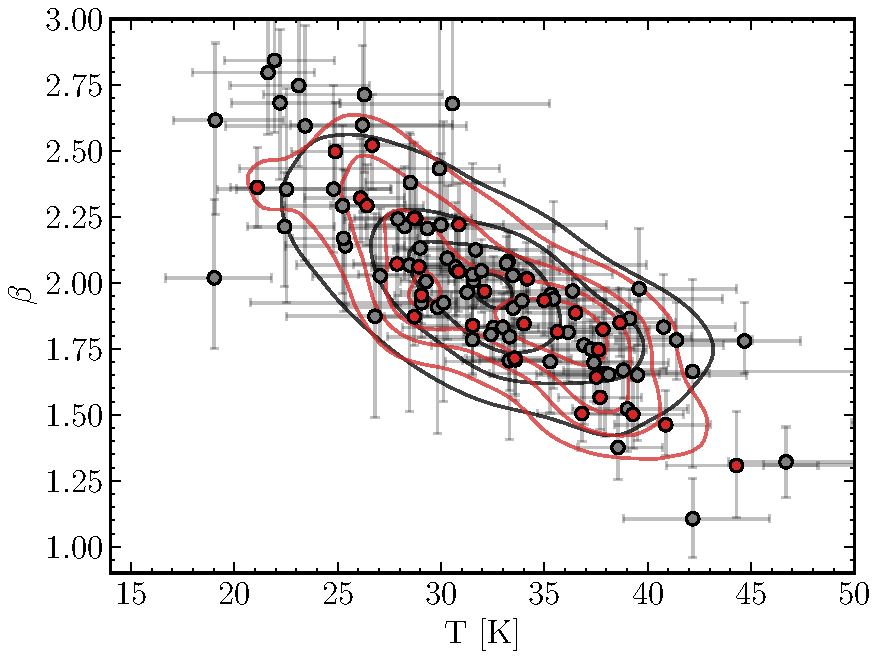
\includegraphics[width=0.8\columnwidth]{Figures/beta_t_correlation.pdf}
	\caption[Relationship between $\beta$ and $T_\textrm{dust}$ for SPT and HerBS galaxies]{Relationship between the dust temperature and the emissivity spectral index for the SPT (black) and HerBS (red) galaxies assuming optically thin dust. The joint posterior distribution for the two sub-samples is shown as contours of the same colour.}
	\label{fig:beta_t_correlation}
\end{figure}

\section{Simulations}
\label{sec:simulations}

In order to assess how accurately our fitting routine derives a galaxy's dust parameters, we ran a suite of mock SEDs with known input parameters and measured how precisely we could recover the dust properties from applying our fitting procedure on our simulated galaxies. We generated our mock galaxies in the following way. First, we assumed that the dust emission can be described by an optically thin, isothermal MBB according to Equation \ref{eq:modified_blackbody_optically_thin}. Next, we produce $2,500$ random SEDs by selecting dust parameters randomly between the lower and upper bounds defined in Table \ref{tab:simulation_inputs}. These values were selected specifically to recreate the width of the posterior distributions observed for real sources. We generated two sets of mock galaxies, one to represent SEDs similar to the real SPT galaxies, and one set that simulates real HerBS galaxies. For the mock HerBS sources we placed each galaxy at a random redshift between $2$ and $4$ and obtained from it flux densities at the same observed wavelengths as for the real HerBS sub-sample (recall Section \ref{sec:sed_fitting}), omitting photometry at $1.2\,$mm as only a few HerBS sources have photometry at this wavelength. In a similar manner, the second sample of mock SPT galaxies were placed at a random redshift between $2$ and $6$, and given the same photometric coverage as a typical SPT galaxy. The $5,000$ SEDs created thus far are models with known inputs; to create observed SEDs, we add flux errors to the models, drawing randomly from a Gaussian distribution with a standard deviation derived from the spread in SNR of real sources at that wavelength. We also assumed a lensing magnification of $5.5$ for SPT galaxies and $5.3$ for HerBS galaxies, in keeping with their median values.

\begin{table}
    \centering
    \begin{tabular}{p{3cm}|p{3cm}}
        \hline
		\hline
        Parameter & Bounds \\
        \hline
        \hline
        log($\mu L_{\textrm{IR}} [L_{\odot}]$) & 13 -- 14 (HerBS) \\
        & 13 -- 14.5 (SPT) \\
		$T_{\textrm{dust}}$ [K] & 20 -- 50 \\
		$\beta$  & 0.5 -- 4 \\
		$\alpha$  & 1 -- 5 \\
        \hline
    \end{tabular}
    \caption[Bounds on the input parameter ranges for mock galaxy simulations]{The upper and lower bounds assumed on the flat priors during the input-output simulations described in Section \ref{sec:simulations}.}
    \label{tab:simulation_inputs}
\end{table}

We added calibration errors in the same manner that we do for the real DSFGs and derived the dust parameters using the same modelling procedure detailed earlier. When fitting we test to see whether the mock galaxy would be detected in our sub-samples (assuming detection limits of $80\,$mJy at $500\,\mu$m for HerBS and $25\,$mJy at $870\,\mu$m for SPT) and remove mock galaxies if they fall to meet the detection limits.

In Figure \ref{fig:in_out_simulations} we show the measured dust properties of the two artificial samples, plotted against their input values. We show the input and output dust masses, dust temperatures and $\beta$ values, all of which are in good agreement, a reflection of the excellent coverage spanning both the thermal peak of dust emission and the Rayleigh - Jeans tail, vital for well constrained $\beta$ values. The root mean sqaure error (RMSE) is calculated for each dust parameter, illustrating the intrinsic scatter that real galaxies have around their "true" values. From these values we know that our real DSFGs recovers their true dust masses to $0.05\,$dex and $0.03\,$dex, dust temperatures to $1.63\,$K and $1.61\,$K and $\beta$ to $0.13$ and $0.09$ for SPT and HerBS galaxies, respectively. The accuracy of the output dust temperatures decreases for warmer temperatures, a result of the SED shifting to shorter wavelengths and the peak being less constrained by the \textit{Herschel} photometry. The right-most panel of the two rows in Figure \ref{fig:in_out_simulations} show the difference in the input and output dust temperatures against the difference in the input and output $\beta$ values. As the mock galaxies are initialized with no intrinsic correlation, the anti-correlation observed here must have been introduced by correlated errors in the two parameters. We measure the RMSE in $\beta$ and $T_\textrm{dust}$ to be approximately $0.1$ and $1.6\,$K, respectively. The RMSE in the $\beta$ and $T_\textrm{dust}$ measurements for real sources (Figure \ref{fig:beta_t_correlation}) are $0.5$ and $8\,$K, respectively. This suggests that the fitting of mock galaxies with no intrinsic correlation does not produce an artificial anti-correlation that can account for the typical RMSE of real galaxies, and thus there is a genuine inverse correlation (of some lesser degree than actually observed in Figure \ref{fig:beta_t_correlation}) between $\beta$ and $T_\textrm{dust}$ that is not caused by correlated measurement errors.

\begin{figure}
	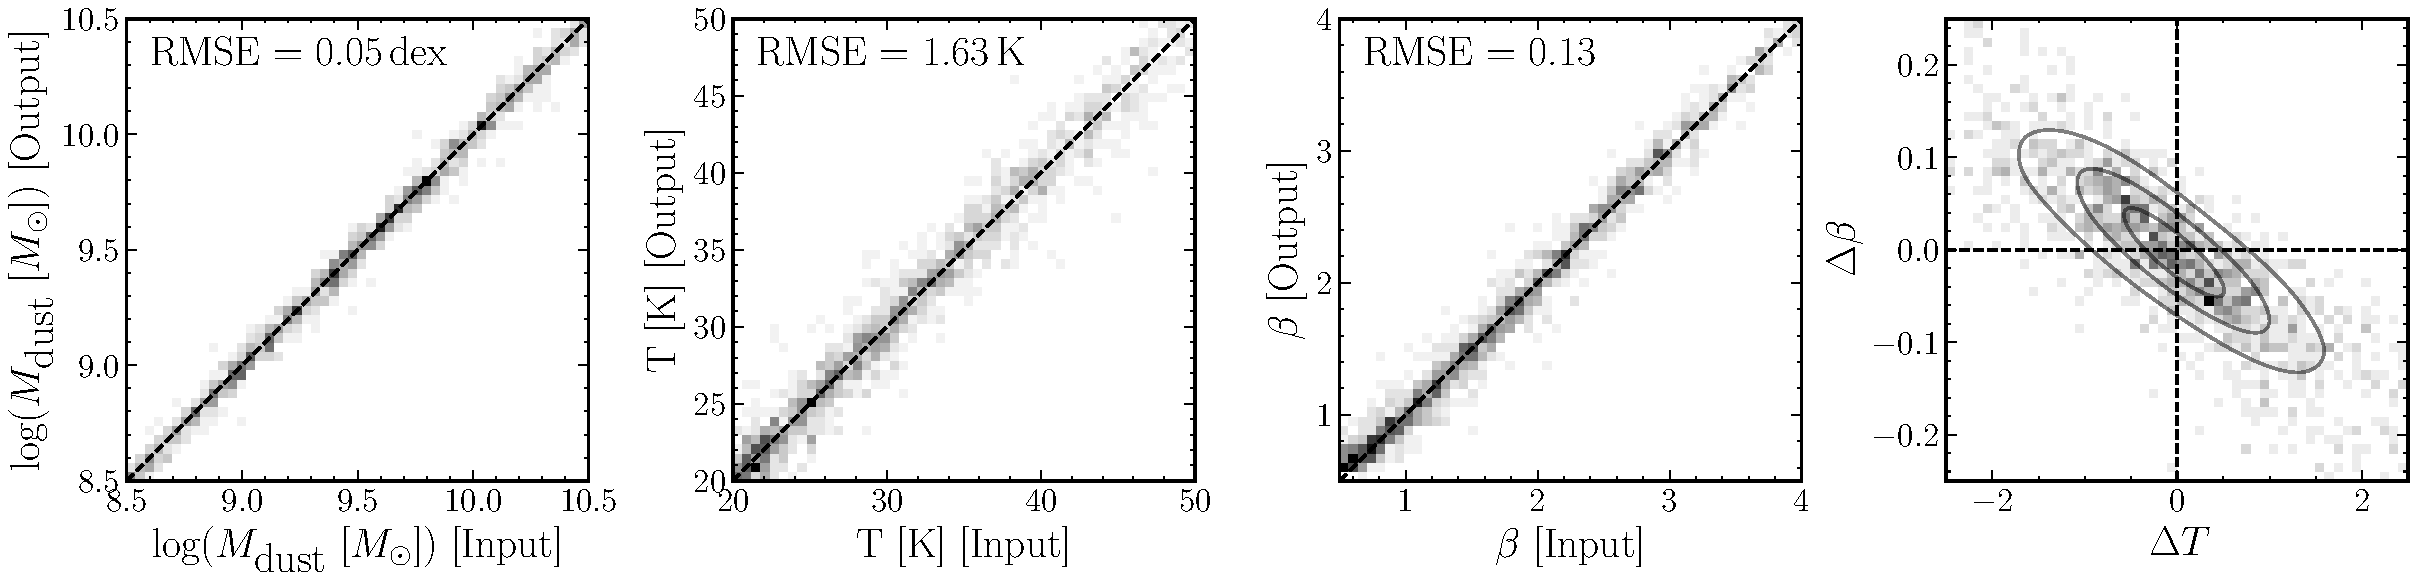
\includegraphics[width=\columnwidth]{Figures/Figure_4_8_part1.pdf}
	\centering
	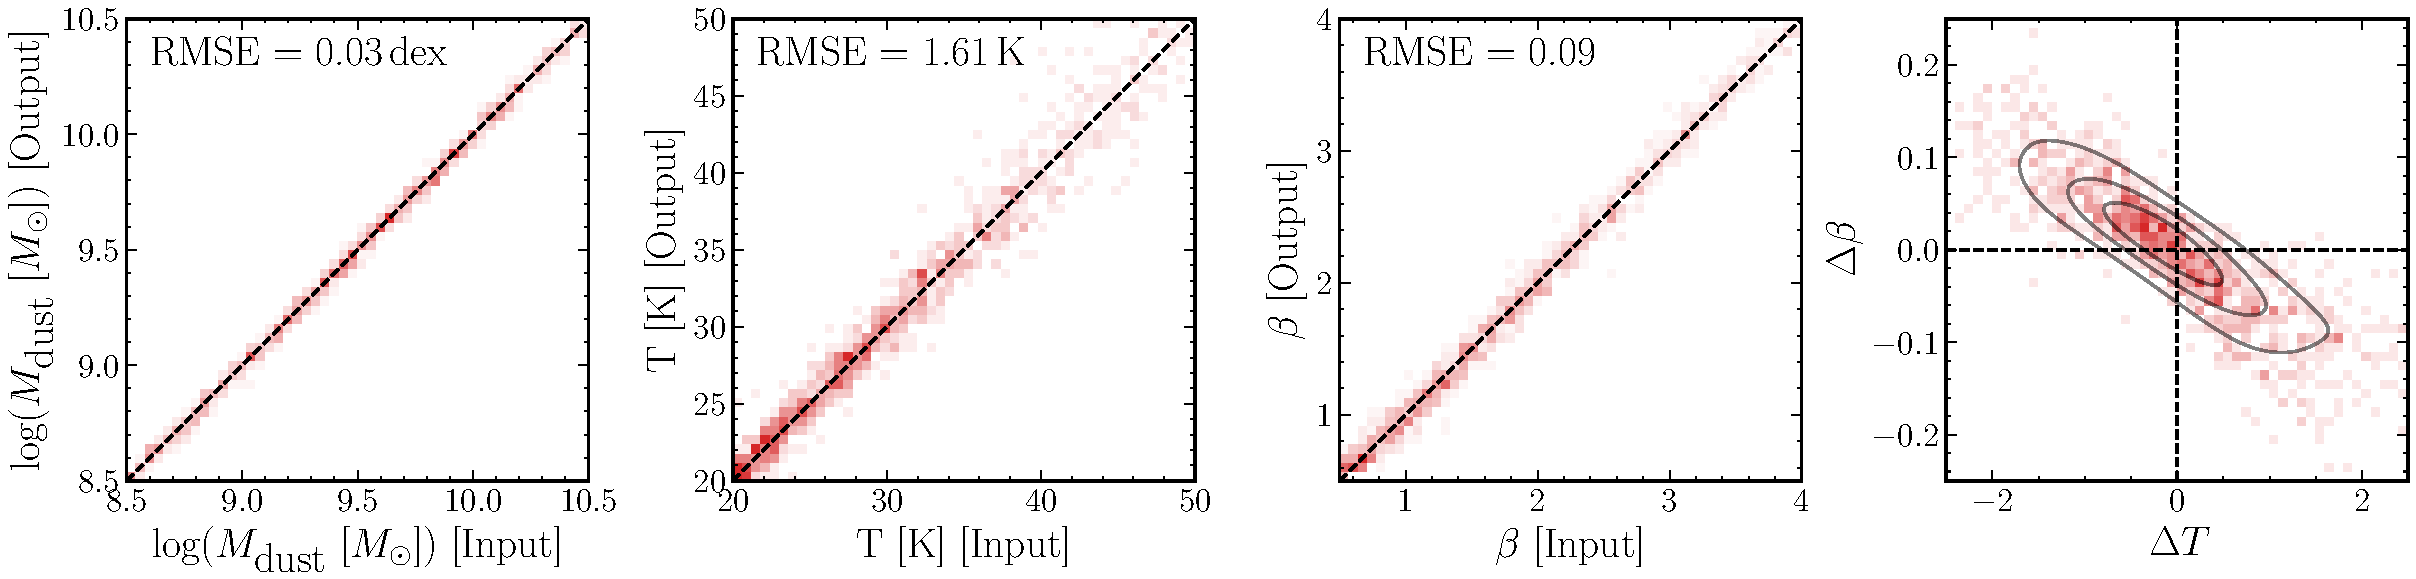
\includegraphics[width=\columnwidth]{Figures/Figure_4_8_part2.pdf}
	\caption[Comparison of the input and output parameter values from simulations]{The input values compared to the measured output values for the simulations described in Section \ref{sec:simulations}. The panels show the following dust parameters: dust mass, dust temperature and dust emissivity index, and the difference between the inputs and outputs in the dust temperature - $\beta$ plane. The top row (black) shows the results of the simulation of SPT galaxies with optically thin dust, while the bottom row (red) represents mock HerBS galaxies.}
	\label{fig:in_out_simulations}
\end{figure}

\section{Evolution of Dust Properties with Redshift}
\label{sec:redshift_evolution}

In this section, we study the redshift evolution of the measured dust properties of HerBS and SPT galaxies in context with low redshift predictions from the Milky Way and local star forming galaxies.

\subsection{Evolution of $\beta$ with Redshift}

Figure \ref{fig:beta_z_evolution} shows the distribution of galaxies in the $\beta-z$ plane. The average value of the dust emissivity spectral index, as measured from the median of each galaxy's posterior distribution in $\beta$, is $1.98$ for SPT and $1.91$ for HerBS galaxies. These values are higher than the values typically assumed in the local Universe. For example, it is significantly higher than the value in our Galaxy, which is uniformly $\beta = 1.51\pm0.01$ across the sky (\citealt{Planck_Collaboration_2015}), and is at the upper end of the range observed for nearby galaxies in JINGLE ($\beta = 0.6 - 2.2$, \citealt{Lamperti_2019}). It is interesting to note, however, that the higher values observed in JINGLE are measured for the most massive galaxies in the sample, which could be the descendants of the DSFGs studied here (\citealt{Eales_2023}, see also Chapter \ref{chapter:Radio_Identifications}). It is difficult to reconcile the $\beta$ values measured for the DSFGs studied here with the values locally, and with the increasing number of recent studies that suggest high redshift galaxies may be better described by an SED with $\beta \sim 2$ (e.g. \citealt{daCunha_2021, Witstok_2023}), we also advocate that future studies of high redshift galaxies adopt this value.

\begin{figure}
	\centering
	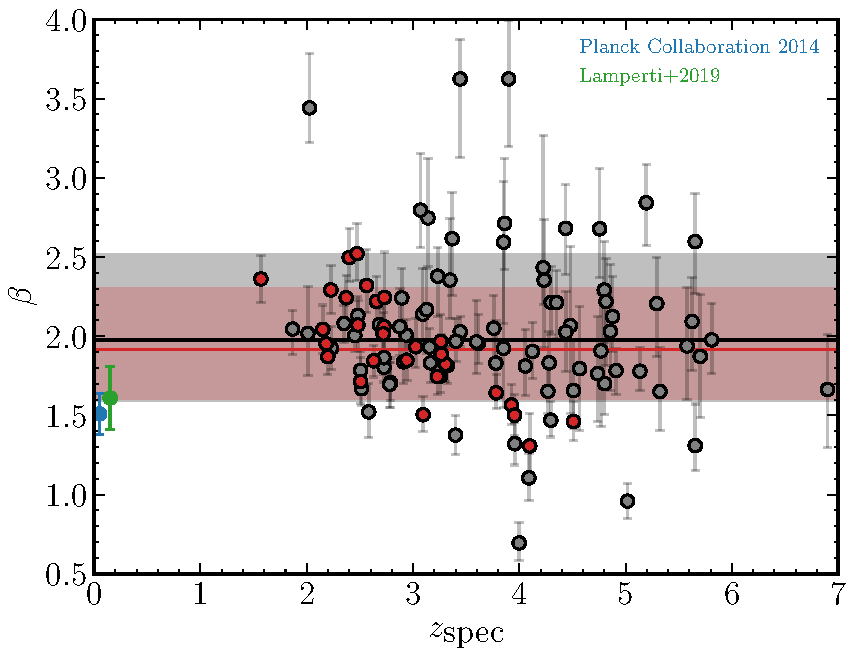
\includegraphics[width=0.8\columnwidth]{Figures/beta_evolution.pdf}
	\caption[Distribution of HerBS and SPT galaxies in the $\beta$ - redshift plane]{The distribution of $\beta$ values for HerBS (red) and SPT (black) galaxies against redshift with the canonical values from the JINGLE survey (green) and the Milky Way (blue). The median value of the stacked posterior distributions are shown as red and black lines for the HerBS and SPT samples respectively, with the shaded regions showing the $16$th to $84$th percentiles.}
	\label{fig:beta_z_evolution}
\end{figure}

Considering the two sub-samples collectively, there is little evidence to suggest that there has been any evolution in $\beta$ over the redshift range $2 < z < 6$. There appears a decreasing trend of $\beta$ with cosmological distance for HerBS galaxies, but this is mostly influenced by the five sources observed at $z \sim 4$. The $500\,\mu$m selection wavelength at $z \sim 4$ is close to the peak in the dust emission, thus biasing us to higher dust temperatures. Given the anti-correlation with $\beta$, it may not be surprising that we observe lower $\beta$ at this redshift for HerBS galaxies. The lack of a redshift evolution in $\beta$ has also been observed in previous studies including \citealt{Ismail_2023} ($2 < z < 3$) and \citealt{Witstok_2023} - a study of $17$ galaxies across $4 < z < 8$.

\subsection{Variation in $\beta$}

While there appears to be no evolution of $\beta$ with redshift, we still observe significant scatter around the average values, which tells us that either measurement errors are scattering values around some common $\beta$, or there is true diversity in the physical and chemical properties of high redshift galaxies. To assess which of these are true, we repeated the simulations from the previous section, except this time we randomly draw $\beta$ values from a uniform distribution that spans the $1\sigma$ range of observed values surrounding the average. This aims to replicate a single population of galaxies with a common $\beta$ value which, if they scatter to a significantly wide distribution after fitting, tells us that the cause is likely measurement errors. The simulations are run in the same way as before, except we now have a narrower range of input beta values ($1.68 - 2.41$ for SPT and $1.61 - 2.26$ for HerBS) and we explore all redshifts between $z = 0$ and $z = 7$.

Figure \ref{fig:beta_z_simulation} shows the difference between the input and output $\beta$ values of these simulations ($1,000$ for each sub-sample), as a function of the input redshift. We find no reason to believe that our fitting procedure underestimates or overestimates the value of $\beta$ at any redshift. For the highest redshift SPT galaxies, the scatter around the "true" $\beta$ appears larger than at $z \sim 0$. However, assuming that the RMSE is approximately equal at all redshifts (which appears to be the case in at least the HerBS galaxies), then we estimate the RMSE on $\Delta \beta$ is $\sim 0.1$ for both sub-samples. The scatter in our measured $\beta$ values in Figure \ref{fig:beta_z_evolution} is $\sim 0.3 - 0.5$, which shows that the measurements errors are smaller than the observed scatter. This implies that the range of $\beta$ observed in Figure \ref{fig:beta_z_evolution} represents a true diversity in the dust properties of DSFGs. The range of $\beta$ that we measure in this study is also not unusually high for high redshift galaxies as the spread in $\beta$ is corroborated by studies such as \citealt{daCunha_2021}, \citealt{Cooper_2022}, \citealt{Ismail_2023} and \citealt{Witstok_2023}.

\begin{figure}
	\centering
	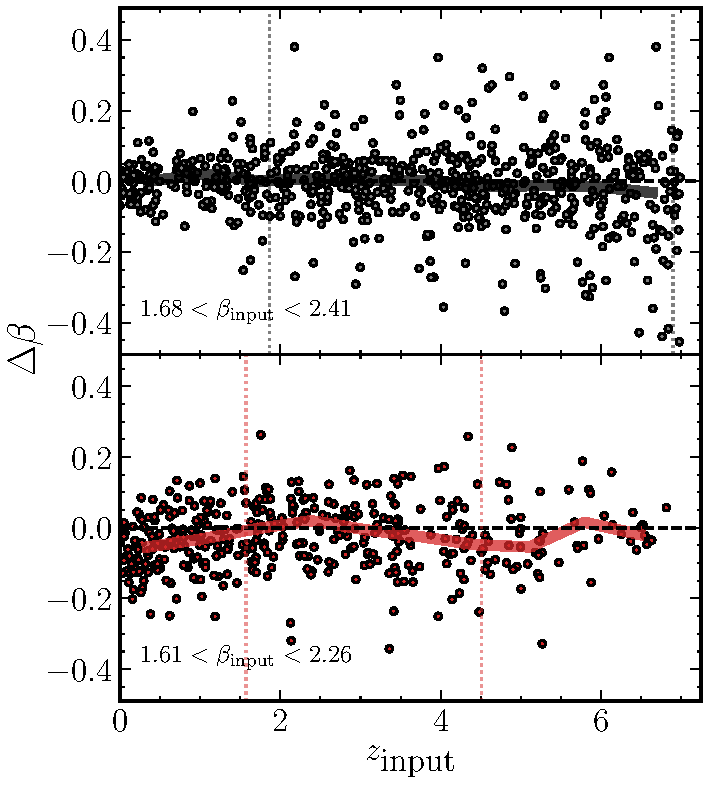
\includegraphics[width=0.8\columnwidth]{figures/beta_simulations.pdf}
	\caption[Difference between input and output $\beta$ from simulations of mock galaxies]{The difference between the input and output $\beta$ values, $\Delta \beta = \beta_{\textrm{output}} - \beta_{\textrm{input}}$, as a function of the input redshift for mock SPT galaxies (top panel) and mock \textit{Herschel} galaxies (bottom panel). Dotted vertical lines represent the minimum and maximum redshift observed in each sample and the thick solid lines represents the median in $\Delta \beta$ as a function of redshift}
	\label{fig:beta_z_simulation}
\end{figure}

A few SPT galaxies have anomalously high $\beta$ ($\gtrsim 2.5$). We mentioned earlier that high values of $\beta$ could arise from the "patchwork" nature of far-IR to mm SEDs, where we combine single-dish observations with interferometric observations with ALMA. To see if the increased spatial resolution of ALMA has split the low resolution sources into multiple components, some of which may subsequently be lost below the ALMA detection threshold at $3\,$mm, we refit a selection of SPT galaxies with high $\beta$ values, removing the ALMA $3\,$mm photometry and assuming $\beta = 2$. These sources are: SPT0112-55 ($\beta = 3.62$), SPT0611-55 ($\beta = 3.44$), SPT2335-53 ($\beta = 2.68$), SPT2340-59 ($\beta = 2.71$) and SPT2349-52 ($\beta = 3.62$). When we then compare the observed $3\,$mm flux density with the predicted value from the $\beta = 2$ MBB, we find that the observed $3\,$mm flux density would need to be $60 - 80\%$ lower than the true flux density to explain such high $\beta$ values. Despite the blending of high redshift galaxies observed in \textit{Herschel} beams (see Chapter \ref{chapter:Radio_Identifications}), this seems unlikely, and the high $\beta$ sources may be genuine.

\subsection{Evolution of $T_{\textrm{dust}}$ with Redshift}
\label{sec:dust_temperature_evolution}

Whether the dust temperature of DSFGs evolves with redshift is a matter of contention in the literature, with studies often claiming completely opposing views. Advocating for hotter dust temperatures at high redshift (e.g. \citealt{Magdis_2012, Magnelli_2014, Swinbank_2014, Bethermin_2015, Faisst_2017, Schreiber_2018, Zavala_2018b, Liang_2019, Ma_2019, Faisst_2020, Bakx_2021, Witstok_2023}), such observational studies are corroborated by the idea that at higher redshifts specific star formation rates (sSFR) and lower dust abundances would lead to hotter dust temperatures. An important caveat to these works is that dust temperature correlates with luminosity (\citealt{Dunne_2000}), which if not adequately accounted for, would naturally lead to a relationship between temperature and redshift. While some studies report a fall in dust temperature (e.g. \citealt{Symeonidis_2013}), most others report little or no evolution (e.g. \citealt{Casey_2018, Jin_2019, Lim_2020a, Dudzeviciute_2020, Reuter_2020, Barger_2022, Drew_2022, Witstok_2023}).

As we showed earlier, the luminosity-weighted dust temperature obtained from SED fitting is dependent on the assumptions we make about the opcaity of the dust. However, the wavelength where the thermal dust emission peaks, $\lambda_\textrm{peak}$, is insensitive to the choice we make, and from Wien's displacement law, we can derive a characteristic dust temperature that we shall name $T_\textrm{peak}$. Neither dust temperature will be the same as the true temperature of the dust in the ISM, but $T_\textrm{peak}$ does allow us to study the evolution in temperature with redshift. 

The top panel of Figure \ref{fig:t_evolution} shows the distribution of SPT and HerBS galaxies in the IR luminosity - redshift plane, along with the detection limits for the two sub-samples assuming a dust temperature of $32\,$K (the median dust temperature of the combined sample) and $\beta = 2$. To avoid any selection effect from the aforementioned luminosity-temperature relationship, we define a small range of IR luminosity for both samples that stays clear of the detection limit (dashed boxes). In the bottom panel of the same figure, we then plot the temperature, as derived from Wien's law, as a function of redshift for the sources in the boxed regions. We compare our measurements of the peak dust temperature ($T_{\textrm{peak}} = 2.898 \times 10^3$ [$\mu$m K]/$\lambda_{\textrm{peak}}$ [$\mu$m]) with the observational relationships derived in the studies of \citealt{Schreiber_2018}, \citealt{Bouwens_2020} and \citealt{Viero_2022}, as well as the median dust temperature of the JINGLE survey. For the combined SPT and HerBS sample there appears little evidence for evolution of temperature with redshift, with peak dust temperatures between $2 < z < 6$ similar to those at $z = 0$ from the observational trends.

\begin{figure}
	\centering
	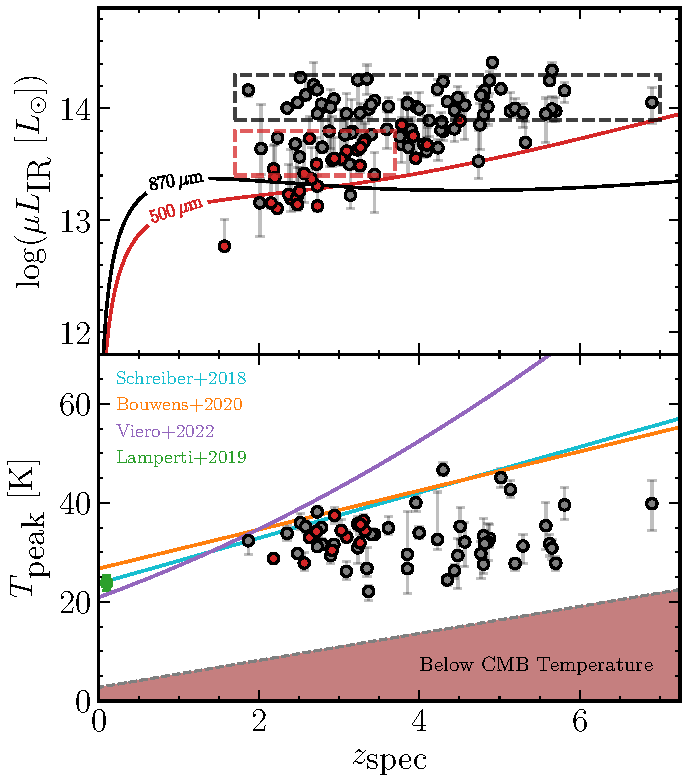
\includegraphics[width=0.75\columnwidth]{Figures/t_evolution.pdf}
	\caption[Distribution of HerBS and SPT galaxies in the $L_{IR} - z$ and $T_\textrm{peak}-z$ planes]{Top panel: the distribution of HerBS (red) and SPT (black) galaxies in the $\mu L_{\textrm{IR}}-z$ plane. The red and black lines represent the detection limit of a HerBS source detected at $> 80\,$mJy ($500\,\mu$m) and an SPT source detected at $> 25\,$mJy ($870\,\mu$m), assuming a dust temperature of $32\,$K and $\beta = 2$. The boxed regions show the limits of our luminosity-limited set of sources from which we test evolutionary trends in the dust temperature. Bottom panel: The distribution of peak dust temperature with redshift for the sources selected in our luminosity-limited subsets. Observed trends from \citealt{Schreiber_2018}, \citealt{Bouwens_2020} and \citealt{Viero_2022} are illustrated as blue, orange and purple lines, respectively. The median dust temperature of local sources from the JINGLE survey is shown as the green error bar.}
	\label{fig:t_evolution}
\end{figure}

\section{Conclusions}

In the previous Chapter we introduced various studies that measure the dust mass density out to high redshifts. This is but one example where our interpretation of galaxy evolution is dependent on the simple assumption that the interstellar dust is the same at all times (specifically that it takes the physical and chemical form of the dust we can observe in the Galaxy and in local galaxies). In this Chapter, we challenged this assumption. We selected roughly $100$ galaxies from HerBS and the SPT-SZ surveys based on photometric coverage at observed wavelengths $>1\,$mm, allowing us to measure well constrained $\beta$ values (as well as ensuring sufficient coverage of the thermal peak in order to constrain the temperature and mass of the dust grains). We modelled the far-IR to millimeter spectra of these galaxies with three models: an optically thin MBB; a general opacity model (which allows for optically thick dust) where the transition between thick and thin is set at $100\,\mu$m; and a third with the transition at $200\,\mu$m. We systematically measured lower masses and higher dust temperatures for the general opacity models but observed no change in the IR luminosities or dust emissivity index. We identified a strong correlation between $\beta$ and dust temperature, which could not be accounted for by the degeneracy between the parameters when fitting the SEDs, suggesting a genuine anti-correlation. We obtained an average value of $\beta = 1.96$, which is higher than in the Galaxy and at the high end of the range observed for local galaxies in JINGLE, although no correlation was observed with redshifts between $z = 2$ and $z = 6$. We advocate for a higher value of $\beta \sim 2$ in future extragalactic studies, as opposed to nominal values between $1.5$ and $1.8$. Finally, we selected a subset of galaxies from both sub-samples with similar luminosities and found that there appears to be no strong evolution in their dust temperatures with redshift.
